% !TEX TS-program = pdflatex
% !TEX encoding = UTF-8 Unicode

% This is a simple template for a LaTeX document using the "article" class.
% See "book", "report", "letter" for other types of document.

\documentclass[11pt]{article} % use larger type; default would be 10pt

\usepackage[utf8]{inputenc} % set input encoding (not needed with XeLaTeX)

%%% Examples of Article customizations
% These packages are optional, depending whether you want the features they provide.
% See the LaTeX Companion or other references for full information.

%%% PAGE DIMENSIONS
\usepackage{geometry} % to change the page dimensions
\geometry{a4paper} % or letterpaper (US) or a5paper or....
\geometry{margin=1in} % for example, change the margins to 2 inches all round
% \geometry{landscape} % set up the page for landscape
%   read geometry.pdf for detailed page layout information

\usepackage{graphicx} % support the \includegraphics command and options

% \usepackage[parfill]{parskip} % Activate to begin paragraphs with an empty line rather than an indent

%%% PACKAGES
\usepackage{booktabs} % for much better looking tables
\usepackage{array} % for better arrays (eg matrices) in maths
\usepackage{paralist} % very flexible & customisable lists (eg. enumerate/itemize, etc.)
\usepackage{verbatim} % adds environment for commenting out blocks of text & for better verbatim
\usepackage{subfig} % make it possible to include more than one captioned figure/table in a single float
% These packages are all incorporated in the memoir class to one degree or another...

%%% HEADERS & FOOTERS
\usepackage{fancyhdr} % This should be set AFTER setting up the page geometry
\pagestyle{plain} % options: empty , plain , fancy
\renewcommand{\headrulewidth}{0pt} % customise the layout...
\lhead{}\chead{}\rhead{}
\lfoot{}\cfoot{\thepage}\rfoot{}

%%% SECTION TITLE APPEARANCE
\usepackage{sectsty}
\allsectionsfont{\sffamily\mdseries\upshape} % (See the fntguide.pdf for font help)
% (This matches ConTeXt defaults)

%%% ToC (table of contents) APPEARANCE
\usepackage[nottoc,notlof,notlot]{tocbibind} % Put the bibliography in the ToC
\usepackage[titles,subfigure]{tocloft} % Alter the style of the Table of Contents
\renewcommand{\cftsecfont}{\rmfamily\mdseries\upshape}
\renewcommand{\cftsecpagefont}{\rmfamily\mdseries\upshape} % No bold!

\usepackage{wasysym}

%%% END Article customizations

%%% The "real" document content comes below...

\title{Systemtest der Backtestingsoftware}
\author{Team Noctua}
%\date{} % Activate to display a given date or no date (if empty),
         % otherwise the current date is printed 

\begin{document}
\maketitle

\section{Algorithmen}
nkd sind minutebars\\
spx sidn daily\\
compq daily\\
Parameter der BTS: \\
Capital \$ 100.000 \\
Transaction Fee \$1 \\ 
Price Premium \$0 \\
Order Sizes 321123 \\
Round Lot Size 100 \\
\newpage
\subsection{SMA gegen Preis}

\begin{center}
\begin{tabular}{ | p{4cm} | p{11cm} |}
\hline 
\textbf{Komponente} & \textbf{Parameter}\\  \hline
Preis & - \\ \hline
SMA & 90 \\ \hline
\end{tabular}
\end{center} 
Bei diesem Algorithmus wird der SMA auf die gegebene Menge an Bars berechnet. Schneidet der Preis den SMA von unten (SMA\textgreater Preis) ist dies ein Kaufsignal, sinkt allerdings der Wert des Preises unter den des SMAs ist dies ein Verkaufssignal. \\

\begin{center}
\begin{tabular}{ | p{5cm} | p{3cm} | p{3cm} | p{3cm} |}
\hline 
Kenndaten & \$SPX & \$COMPQ &  \$NKD \\ \hline
Net Worth [\$]&   & &  \\ \hline
Portfolio Performance [\%]& & &  \\ \hline
Sharpe Ratio& & &  \\ \hline
Mean Deviation of Portfolio Performance [\%]& & &  \\ \hline
Mean Deviation of Equity Price [\$]& & &  \\ \hline
Return on Investment [\%]& & &  \\ \hline
Number of Good Trades& & &  \\ \hline
Gain From Good Trades [\$]& & &  \\ \hline
Number of Bad Trades& & &  \\ \hline
Loss From Bad Trades [\$]& & &  \\ \hline
Ratio of Good Trades& & &  \\ \hline
\end{tabular}
\end{center}

\begin{figure}[h]
 \centering
  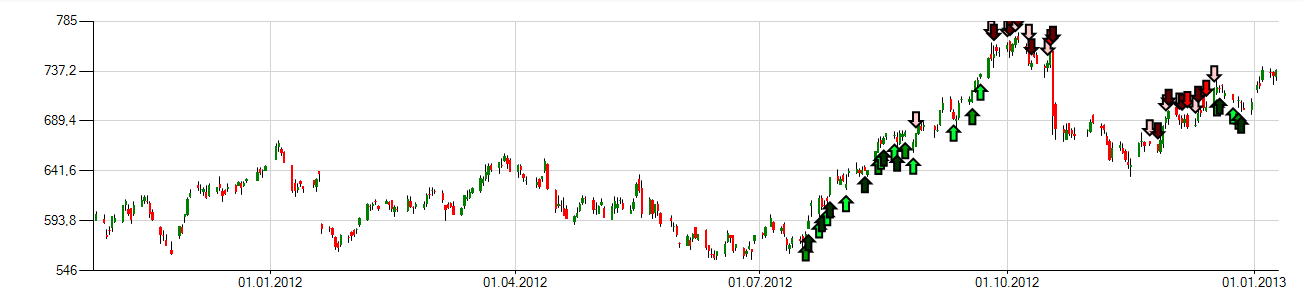
\includegraphics[width=1\textwidth]{images/Tests/test.png}
 \caption{Testbild}
 \label{fig:testbild}
\end{figure}

\textbf{Interpretation} \\
Interpretation von den Sachen die ich seh.Interpretation von den Sachen die ich seh.Interpretation von den Sachen die ich seh.Interpretation von den Sachen die ich seh.Interpretation von den Sachen die ich seh.Interpretation von den Sachen die ich seh.Interpretation von den Sachen die ich seh.Interpretation von den Sachen die ich seh.Interpretation von den Sachen die ich seh.Interpretation von den Sachen die ich seh.Interpretation von den Sachen die ich seh.
\newpage
\end{document}
